\documentclass[a4paper]{article}
\usepackage[
	pdftex,
	colorlinks=true,
	bookmarksnumbered=true,
	bookmarksopen=true,
	bookmarksopenlevel=3,
	pdfstartview=FitP,
	urlcolor=blue,
]{hyperref}
\pdfinfo{
	/Title(Esercitazione di Laboratorio: Arduino)
	/Author(Coa Giulio, Licastro Dario, Montano Alessandra)
}
\usepackage[italian]{babel}
\usepackage{amsmath,geometry,graphicx,listings,mdsymbol,stmaryrd,subcaption,titling,xcolor}
\definecolor{comment}{rgb}{1, 0.83, 0}
\lstset{
	backgroundcolor = \color{white},
	basicstyle = \ttfamily \footnotesize \color{black},
	breakatwhitespace = false,
	breaklines = true,
	captionpos = b,
	columns = flexible,
	commentstyle = \color{comment},
	escapeinside = {\%*}{*)},
	frame = tb,
	keepspaces = true,
	keywordstyle = \color{blue},
	language = C++,
	numbers = left,
	numbersep = 5pt,
	numberstyle = \tiny\color{black},
	showspaces = false,
	showstringspaces = false,
	showtabs = false,
	stepnumber = 1,
	stringstyle = \color{red},
	tabsize = 4
}
\graphicspath{{./Image/}}
\renewcommand\maketitlehooka{
	\null
	\mbox{}
	\vfill
}
\renewcommand\maketitlehookd{
	\vfill
	\null
}
\newcommand\abs[1]{\left|#1\right|}
\title{
	\begin{center}
		Esercitazione di Laboratorio:
	\end{center}
	\newline
	\begin{center}
		Arduino
	\end{center}
}
\author{
	Coa Giulio (s236723)
	\and
	Licastro Dario (s234421)
	\and
	Montano Alessandra (s238160)
}
\begin{document}
	%-----------------------------------------------------------------------------
	%  TITLE
	%-----------------------------------------------------------------------------
	\begin{titlingpage}
		\maketitle
	\end{titlingpage}
	\newpage
	%-----------------------------------------------------------------------------
	%  PURPOSE OF THE EXPERIENCE
	%-----------------------------------------------------------------------------
	\section{Scopo dell'esperienza}
		Lo scopo di questa esercitazione è sviluppare un termometro digitale tramite l'uso di un sensore di temperatura e di una scheda Arduino.
	%-----------------------------------------------------------------------------
	%  INSTRUMENTATION USED
	%-----------------------------------------------------------------------------
	\section{Strumentazione utilizzata}
		La strumentazione usata durante l'esercitazione è:
		\begin{center}
			\begin{tabular}{ |c|c|c| }
				\hline
				\multirow{\textbf{Strumento}}	 		   & \textbf{Marca e Modello} & \textbf{Caratteristiche} \\
				\hline
				\multirow{Multimetro}			 		   & Agilent 34401A			  & \\
				\multirow{Oscilloscopio}		 		   & Rigol DS1054Z			  & 4 canali, \\
												 		   &						  & $ B = 50 \, \mathrm{MHz} $, \\
												 		   &						  & $ f_{\mathrm{c}} = 1 \, \mathrm{G\frac{Sa}{s}} $, \\
												 		   &						  & $ R_{\mathrm{i}} = 1 \, \mathrm{M\Omega} $, \\
												 		   &						  & $ C_{\mathrm{i}} = 13 \, \mathrm{pF} $, \\
												 		   &						  & $ 12 \, \mathrm{Mbps} $ di profondità di memoria \\
				\multirow{Generatore di segnali} 		   & Rigol DG1022			  & 2 canali, \\
												 		   &						  & $ f_{\mathrm{uscita}} = 20 \, \mathrm{MHz} $, \\
												 		   &						  & $ Z_{\mathrm{uscita}} = 50 \, \mathrm{\Omega} $ \\
				\multirow{Scheda Arduino}	 		   	   & UNO					  & $ f_{\mathrm{c, max}} = 76.9 \, \mathrm{k\frac{Sa}{s}} $ \\
				\multirow{Sensore di temperatura}	 	   & LM335					  & $ S = 10 \, \mathrm{m\frac{V}{K}} $, \\
														   &						  & $ V_{\mathrm{out}} = 0 \, \mathrm{V} $ @ $ 0 \, \mathrm{K} $ \\
														   &						  & $ \delta T = \pm 2 \, \mathrm{\text{\textdegree}C} $ \\
														   &						  & Campo di temperatura pari a $ -40 \div 100 \, \mathrm{\text{\textdegree}C} $ \\
														   &						  & Resistenza termica pari a $ 165 \, \mathrm{\frac{\text{\textdegree} C}{W}} $ \\
				\multirow{Cavi coassiali}		 		   &						  & Capacità dell'ordine dei $ 80 \div 100 \, \mathrm{p\frac{F}{m}} $ \\
				\multirow{Connettori}			 		   &						  & \\
				\hline
			\end{tabular}
		\end{center}
	%-----------------------------------------------------------------------------
	%  THEORETICAL PREMISES
	%-----------------------------------------------------------------------------
	\section{Premesse teoriche}
		\subsection{Incertezza sulla misura dell'oscilloscopio}
			La misura del valore di un segnale tramite l’oscilloscopio (sia esso l'ampiezza, la frequenza, il periodo, etc.) presenta un'incertezza che dipende, principalmente, da due fattori:
			\begin{itemize}
				\item l’incertezza strumentale introdotta dall’oscilloscopio (ricavabile dal manuale).
				\item l’incertezza di lettura dovuta all’errore del posizionamento dei cursori.
			\end{itemize}
			Quest’ultima incertezza deriva dal fatto che il segnale visualizzato non ha uno spessore nullo sullo schermo.
		\subsection{Arduino}
			Arduino è una piattaforma elettronica open surce basata su un hardware di facile utilizzo e programmabie in un ambiente software dedicato.
			\subsubsection{Arduino UNO}
				Arduino UNO è una scheda composta da un convertitore ADC a $ 10 $ bit ($ 8 $ bit se la frequenza d'utilizzo è maggiore di $ 15 \, \mathrm{k\frac{Sa}{s}} $) che può essere alimentato da due distinte sorgenti, una interna alla scheda da $ 1.1 \pm 0.1 \, \mathrm{V} $ e una esterna da $ 5 \pm 0.25 \, \mathrm{V} $ ($ 4.85 \pm 0.4 \, \mathrm{V} $ se si usa la porta USB 3.0 anzichè la porta USB 2.0).
				\begin{figure}[h!]
					\centering
					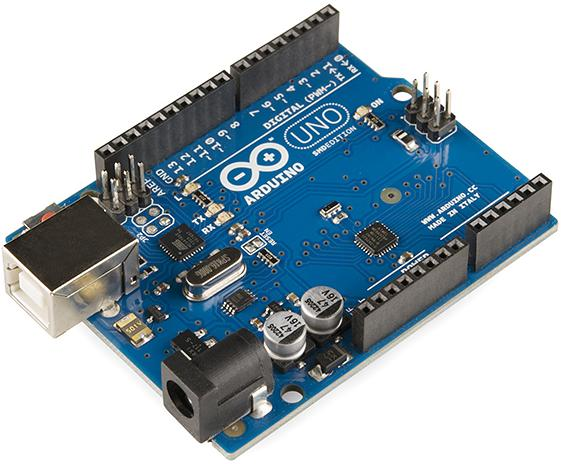
\includegraphics[scale=0.6]{ArduinoUNO}
					\caption{Arduino UNO.}
					\label{fig:ArduinoUNO}
				\end{figure}
		\subsection{Sensore LM335}
			Il sensore LM335 è un sensore di temperatura prodotto dalla National Semiconductor; esso permette di avere in uscita una tensione proporzionale alla temperatura rilevata ($ V_{\mathrm{out}} = S \cdot T_{\mathrm{K}} $).
			\newline
			Il suo comportamento è assimilabile a quello di un diodo di Zener la cui corrente $ I_{\mathrm{D}} $ deve essere compresa nell'intervallo $ 0.4 \, \mathrm{mA} \div 5 \, \mathrm{mA} $.
			\begin{figure}[h!]
				\centering
				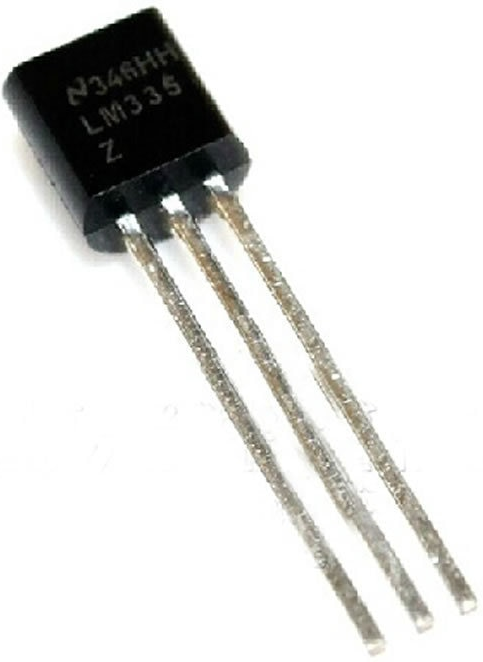
\includegraphics[scale=0.2]{LM335}
				\caption{Sensore LM335.}
				\label{fig:LM335}
			\end{figure}
	%-----------------------------------------------------------------------------
	%  LABORATORY EXPERIENCE
	%-----------------------------------------------------------------------------
	\section{Esperienza in laboratorio}
		\subsection{Circuito di condizionamento}
			Per i nostri scopi, il sensore LM335 deve lavorare lavorare in regione di polarizzazione inversa, percui esso verrà utilizzato con il catodo collegato alla massa e con l'anodo collegato alla sorgente di tensione.
			\newline
			Al fine di garantire un corretto funzionamento del sensore, dobbiamo garantire che la corrente che vi circola all'interno sia nel range di funzionamento; a tale scopo applichiamo una resistenza $ R_{1} $ a monte del diodo, di modo che la corrente che scorra nel diodo rientri nel suddetto range.
			\begin{figure}[h!]
				\centering
				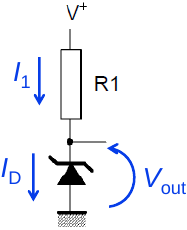
\includegraphics[scale=0.5]{circuitoDiCondizionamento}
				\caption{Circuito di condizionamento.}
				\label{fig:circuitoDiCondizionamento}
			\end{figure}
		\subsection{Misura della temperatura}
			Successivamente, abbiamo collegato il sensore all'Arduino UNO, seguendo lo schema nella figura seguente ed impostando una tensione d'alimentazione $ V_{\mathrm{cc}} $ pari a $ 4.85 \pm 0.4 \, \mathrm{V} $.
			\begin{figure}[h!]
				\centering
				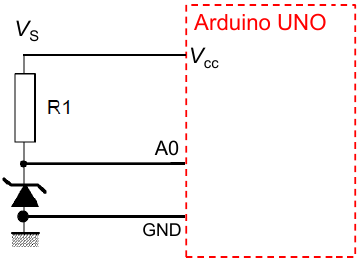
\includegraphics[scale=0.5]{collegamentoCircuitoArduino}
				\label{fig:collegamentoCircuitoArduino}
			\end{figure}
			\newline
			L'Arduino UNO produce, in uscita, un valore numerico nell'intervallo $ 0 \div 1023 $ ($ 0 \div 2^{N_{\mathrm{B}}} - 1 $); al fine di ottenere la temperatura di lavoro del sensore, abbiamo usato la funzione
			\begin{center}
				$ T_{\mathrm{K}} = D_{\mathrm{out}} \cdot \frac{V_{\mathrm{FR}}}{2^{N_{\mathrm{B}}}} \cdot \frac{1}{S} $
			\end{center}
			Mentre, per ottenere la tensione ad essa associata, abbiamo sfruttato la relazione $ V_{\mathrm{out}} = S \cdot T_{\mathrm{K}} $, ottenendo la formula
			\begin{center}
				$ V_{\mathrm{out}} = D_{\mathrm{out}} \cdot \frac{V_{\mathrm{FR}}}{2^{N_{\mathrm{B}}}} $
			\end{center}
			Queste formule sono state implementate nel seguente codice, simil \verb!C++!, che è stato usato per settare l'Arduino UNO.
			\newpage
			\lstinputlisting[language = C++, label = {lst:arduinoCode}]{arduinoCode.cpp}
		\subsection{Stima dell'incertezza}
			Al fine di determinare l'incertezza assoluta associata alla misura di temperatura ottenuta, abbiamo applicato la formula di propagazione delle incertezze del modello deterministico.
			\begin{center}
				$ y = f(x_{1}, x_{2}, \ \dots \ , x_{\mathrm{m}}) $
			\end{center}
			\begin{center}
				$$ \delta y = \sum_{i=1}^{m} \abs{\frac{\partial f}{\partial x_{\mathrm{i}}}} \cdot \delta x_{\mathrm{i}} $$
			\end{center}
			Il valore ottenuto è molto elevato, percui tale misura non si può considerare affidabile.
		\subsection{Modifica del circuito di condizionamento}
			Al fine di ridurre l'incertezza associata a tale misurazione, imponiamo che la tensione di fondo scala $ V_{\mathrm{FR}} $ sia pari al riferimento interno $ V_{\mathrm{int}} $ dell'Arduino UNO; questa tensione è nota con un'incertezza assoluta minore e, pertanto, risulta essere più accurata.
			\newline
			Per poter applicare questa soluzione, occorre portare la tensione $ V_{\mathrm{out}} $ dal range attuale ($ 0 \div 5 \, \mathrm{V} $) al range $ 0 \div 1.1 \, \mathrm{V} $; a tale scopo, applichiamo un partitore di tensione in parallelo al sensore.
			\begin{figure}[h!]
				\centering
				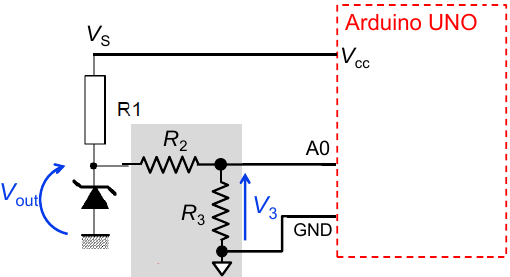
\includegraphics[scale=0.5]{collegamentoCircuitoArduinoPartitore}
				\label{fig:collegamentoCircuitoArduinoPartitore}
			\end{figure}
			\newpage
			Tale partitore deve essere strutturato di modo da
			\begin{itemize}
				\item Minimizzare gli effetti di carico.
				\item Imporre una tensione $ V_{3} $ di, massimo, $ 1.1 \, \mathrm{V} $.
				\item Non assorbire troppa corrente, pena il corretto funzionamento del sensore.
				\item Attenuare la tensione $ V_{\mathrm{out}} $ di un fattore $ \ge 3 $
			\end{itemize}
			A tale scopo le resistenze $ R_{2} $ ed $ R_{3} $ devono essere abbastanza elevate per portare alla saturazione in caso di tensioni maggiori di $ 1.1 \, \mathrm{V} $, ma devono essere abbastanza piccole per evitare di assorbire troppa corrente.
			\newline
			L'inserimento di questo partitore si ripercuote sulla funzione usata per determinare la temperatura di lavoro del sensore e la tensione che esso produce in output; nello specifico, esse diventano
			\begin{center}
				$ T_{\mathrm{K}} = D_{\mathrm{out}} \cdot \frac{V_{\mathrm{FR}}}{2^{N_{\mathrm{B}}}} \cdot \frac{1}{S} \cdot (1 + \frac{R_{2}}{R_{3}}) $
			\end{center}
			\begin{center}
				$ V_{\mathrm{out}} = D_{\mathrm{out}} \cdot \frac{V_{\mathrm{FR}}}{2^{N_{\mathrm{B}}}} \cdot (1 + \frac{R_{2}}{R_{3}}) $
			\end{center}
			Queste formule sono state implementate nel codice che è stato presentato al punto \ref{lst:arduinoCode}.
			\newline
			Una volta eseguite queste modifiche al circuito, abbiamo ripetuto l'esperienza, misurando nuovamente la temperatura di lavoro del sensore, la tensione che esso produce in uscita e l'incertezza associata alla misura.
	%-----------------------------------------------------------------------------
	%  RESULTS
	%-----------------------------------------------------------------------------
	\section{Risultati}
		\subsection{Circuito di condizionamento}
			In base ai dati fornitici, abbiamo proceduto al calcolo della tensione massima e della tensione minima a cui il sensore LM335 deve lavorare.
			\begin{equation*}
				\begin{split}
					V_{\mathrm{out, max}} &= S \cdot T_{\mathrm{K, max}} = \\
										  &= S \cdot (T_{\mathrm{max}} + 273.15) = \\
										  &= 10m \cdot (50 + 273.15) = \\
										  &= 3.23 \, \mathrm{V}
				\end{split}
			\end{equation*}
			\begin{equation*}
				\begin{split}
					V_{\mathrm{out, min}} &= S \cdot T_{\mathrm{K, min}} = \\
										  &= S \cdot (T_{\mathrm{min}} + 273.15) = \\
										  &= 10m \cdot (5 + 273.15) = \\
										  &= 2.78 \, \mathrm{V}
				\end{split}
			\end{equation*}
			Essendo che la resistenza $ R_{1} $ è posta in serie al sensore, la corrente che scorre nel diodo è uguale a quella che scorre nella resistenza (in realtà è approssimabile, dato che si va a misurare la tensione ai capi del diodo e si ha un minimo di "perdite").
			\begin{center}
				$ I_{\mathrm{D}} \approx I_{1} = \frac{V_{\mathrm{s}} - V_{\mathrm{out}}}{R_{1}} $
			\end{center}
			Da ciò, si ha che le limitazioni sulla corrente che attraversa il diodo diventano
			\begin{center}
				$ \frac{V_{\mathrm{s}} - V_{\mathrm{out, max}}}{R_{1}} > 0.4 \, \mathrm{mA} $
			\end{center}
			\begin{center}
				$ \frac{V_{\mathrm{s}} - V_{\mathrm{out, min}}}{R_{1}} < 5 \, \mathrm{mA} $
			\end{center}
			Da cui si ha che
			\begin{center}
				$ \frac{V_{\mathrm{s}} - V_{\mathrm{out, max}}}{0.4m} > R_{1} > \frac{V_{\mathrm{s}} - V_{\mathrm{out, min}}}{5m} $
			\end{center}
			\begin{center}
				$ 4050 \, \mathrm{\Omega} > R_{1} > 414 \, \mathrm{\Omega} $
			\end{center}
			Successivamente, abbiamo stimato la temperatura dell'ambiente in cui il diodo avrebbe lavorato, tenendo conto dell'autoriscaldamento del sensore, e, di conseguenza, la tensione in uscita che esso avrebbe prodotto.
			\begin{equation*}
				\begin{split}
					V_{\mathrm{out}} &= S \cdot T_{\mathrm{K}} = \\
									 &= S \cdot (T + 273.15) = \\
									 &= 10m \cdot (25 + 273.15) = \\
									 &= 2.98 = \\
									 &\approx 3 \, \mathrm{V}
				\end{split}
			\end{equation*}
			Ed abbiamo imposto che $ I_{\mathrm{D}} $ fosse di $ 2 \, \mathrm{mA} $, da cui
			\begin{equation*}
				\begin{split}
					R_{1} &= \frac{V_{\mathrm{s}} - V_{\mathrm{out}}}{I_{1}} = \\
						  &= \frac{4.85 - 3}{2m} = \\
						  &= 925 \, \mathrm{\Omega}
				\end{split}
			\end{equation*}
		\subsection{Misura della temperatura} 
			Il valore di $ D_{\mathrm{out}} $ ottenuto è pari a $ 606 $, percui la temperatura a cui lavora il sensore sarà
			\begin{equation*}
				\begin{split}
					T_{\mathrm{K}} &= D_{\mathrm{out}} \cdot \frac{V_{\mathrm{FR}}}{2^{N_{\mathrm{B}}}} \cdot \frac{1}{S} = \\
								   &= 606 \cdot \frac{4.85}{2^{10}} \cdot \frac{1}{10m} = \\
								   &= 286.55 \, \mathrm{K}
				\end{split}
			\end{equation*}
			\begin{equation*}
				\begin{split}
					T &= T_{\mathrm{K}} - 273.15 = \\
					  &= 286.55 - 273.15 = \\
					  &= 13.40 \, \mathrm{\text{\textdegree} C}
				\end{split}
			\end{equation*}
			Mentre la tensione in uscita sarà
			\begin{equation*}
				\begin{split}
					V_{\mathrm{out}} &= D_{\mathrm{out}} \cdot \frac{V_{\mathrm{FR}}}{2^{N_{\mathrm{B}}}} = \\
									 &= 606 \cdot \frac{4.85}{2^{10}} = \\
									 &= 2.87 \, \mathrm{V}
				\end{split}
			\end{equation*}
		\subsection{Stima dell'incertezza}
			Come detto precedentemente, abbiamo applicato la formula di propagazione delle incertezze del modello deterministico, ottenendo un'incertezza pari a
			\begin{equation*}
				\begin{split}
					\delta T &= \abs{\frac{\partial T}{\partial D_{\mathrm{out}}}} \cdot \delta D_{\mathrm{out}} + \abs{\frac{\partial T}{\partial V_{\mathrm{FR}}}} \cdot \delta V_{\mathrm{FR}} + \abs{\frac{\partial T}{\partial S}} \cdot \delta S = \\
							 &= \frac{V_{\mathrm{FR}}}{S \cdot 2^{N_{\mathrm{B}}}} \cdot \delta D_{\mathrm{out}} + \frac{D_{\mathrm{out}}}{S \cdot 2^{N_{\mathrm{B}}}} \cdot \delta V_{\mathrm{FR}} + \delta T^{sensor} = \\
							 &= \frac{4.85}{10m \cdot 2^{10}} \cdot \delta D_{\mathrm{out}} + \frac{606}{10m \cdot 2^{10}} \cdot 0.4 + 2 = \\
							 &= 1 + \frac{606}{10m \cdot 2^{10}} \cdot 0.4 + 2 = \\
							 &= XXXX \, \mathrm{K}
				\end{split}
			\end{equation*}
		\subsection{Modifica del circuito di condizionamento}
			Essendo che il partitore deve attenuare di un fattore $ \ge 3 $ la tensione $ V_{\mathrm{out}} $, si ha che
			\begin{equation*}
				\begin{split}
					&V_{3} \le \frac{V_{\mathrm{out}}}{3} \\
					&V_{3} \le \frac{3}{3} \\
					&V_{3} \le 1 \, \mathrm{V}
				\end{split}
			\end{equation*}
			Sfruttando questo vincolo, imponiamo che $ V_{3} $ sia pari a $ 1 \, \mathrm{V} $, ovvero, imponiamo che
			\begin{equation*}
				\begin{split}
					V_{3} &= \frac{R_{3}}{R_{2} + R_{3}} \cdot V_{\mathrm{s}} \\
					\frac{R_{3}}{R_{2} + R_{3}} &= \frac{V_{3}}{V_{\mathrm{s}}} = \\
												&= \frac{1}{4.85} = \\
												&= 0.21
				\end{split}
			\end{equation*}
			Questa relazione non identifica univocamente le resistenze del partitore e, pertanto, ci lascia un certo grado di libertà nella progettazione del circuito; nell'ottica di scegliere delle resistenze che consentissero di non avere un partitore che assorba troppa corrente, abbiamo scelto le resistenze coi seguenti valori
			\begin{center}
				$ R_{2} = 3.8 \, \mathrm{k\Omega} $
			\end{center}
			\begin{center}
				$ R_{3} = 1 \, \mathrm{k\Omega} $
			\end{center}
			L'inserimento del partitore non ci porta a dover ristrutturare il circuito, in quanto la corrente che scorre nel sensore è sufficiente a farlo funzionare.
			\begin{equation*}
				\begin{split}
					I_{\mathrm{D}} &= I_{\mathrm{D, old}} - \frac{V_{\mathrm{out}}}{R_{2} + R_{3}} = \\
						  &= 2m - \frac{3}{3.8k + 1k} = \\
						  &= 1.38 \, \mathrm{mA}
				\end{split}
			\end{equation*}
			Il valore di $ D_{\mathrm{out}} $ ottenuto è pari a $ XXXX $, percui la temperatura a cui lavora il sensore sarà
			\begin{equation*}
				\begin{split}
					T_{\mathrm{K}} &= D_{\mathrm{out}} \cdot \frac{V_{\mathrm{FR}}}{2^{N_{\mathrm{B}}}} \cdot \frac{1}{S} \cdot (1 + \frac{R_{2}}{R_{3}}) = \\
								   &= XXXX \cdot \frac{1.1}{2^{10}} \cdot \frac{1}{10m} \cdot (1 + \frac{3.8k}{1k}) = \\
								   &= XXXX \, \mathrm{K}
				\end{split}
			\end{equation*}
			\begin{equation*}
				\begin{split}
					T &= T_{\mathrm{K}} - 273.15 = \\
					  &= XXXX - 273.15 = \\
					  &= XXXX \, \mathrm{\text{\textdegree} C}
				\end{split}
			\end{equation*}
			Mentre la tensione in uscita sarà
			\begin{equation*}
				\begin{split}
					V_{\mathrm{out}} &= D_{\mathrm{out}} \cdot \frac{V_{\mathrm{FR}}}{2^{N_{\mathrm{B}}}} \cdot (1 + \frac{R_{2}}{R_{3}}) = \\
									 &= XXXX \cdot \frac{1.1}{2^{10}} \cdot (1 + \frac{3.8k}{1k}) = \\
									 &= XXXX \, \mathrm{V}
				\end{split}
			\end{equation*}
			L'incertezza associata a questa misurazione è
			\begin{equation*}
				\begin{split}
					\delta T &= \abs{\frac{\partial T}{\partial D_{\mathrm{out}}}} \cdot \delta D_{\mathrm{out}} + \abs{\frac{\partial T}{\partial V_{\mathrm{FR}}}} \cdot \delta V_{\mathrm{FR}} + \abs{\frac{\partial T}{\partial S}} \cdot \delta S = \\
							 &= \frac{V_{\mathrm{FR}}}{S \cdot 2^{N_{\mathrm{B}}}} \cdot \delta D_{\mathrm{out}} + \frac{D_{\mathrm{out}}}{S \cdot 2^{N_{\mathrm{B}}}} \cdot \delta V_{\mathrm{FR}} + \delta T^{sensor} = \\
							 &= \frac{1.1}{10m \cdot 2^{10}} \cdot \delta D_{\mathrm{out}} + \frac{XXXX}{10m \cdot 2^{10}} \cdot 0.1 + 2 = \\
							 &= 1 + \frac{XXXX}{10m \cdot 2^{10}} \cdot 0.1 + 2 = \\
							 &= XXXX \, \mathrm{K}
				\end{split}
			\end{equation*}
			Come si può notare, essa è minore dell'incertezza associata alla precedente misurazione, pertanto questa misura è più affidabile della precedente.
\end{document}
